\documentclass[12pt]{report}
\usepackage[utf8x]{inputenc}
\usepackage{graphicx}
\usepackage{textcomp, gensymb}
\usepackage{gensymb}
\usepackage{amssymb}
\usepackage{algorithm}
\usepackage[noend]{algpseudocode}
\usepackage{algpseudocode}
\graphicspath{{./images}}
\usepackage{fancyhdr}
\usepackage{blindtext}
\usepackage[colorlinks=true, urlcolor=black, linkcolor=black]{hyperref}
\hypersetup{
colorlinks=true,
linkcolor=black,
urlcolor=black
}
\usepackage{url}


\title{ETERNITY:FUNCTION F4}
\author{Tavtej Singh Lehri}
\date{}
\newcommand*{\Gtr}{\smallrel\gtr}

\makeatletter
\let\thetitle\@title
\let\theauthor\@author
\let\thedate\@date
\makeatother

\fancypagestyle{}{}
\fancyhf{}
\rhead{\thetitle}
\cfoot{\thepage}

\begin{document}

\begin{titlepage}
\centering
\vspace*{0.5 cm}

\begin{center}
\textsc{\Large CONCORDIA UNIVERSITY}\\ [2.0 cm]    
\end{center}

\textsc{\large SOEN 6011: Software Engineering Processes}\\[0.5 cm]
\rule{\linewidth}{0.2 mm}\\[0.4 cm]
{\LARGE \textbf \thetitle}\\[0.2 cm]
{\LARGE \textbf{$\Gamma$(x)}}
\rule{\linewidth}{0.2 mm}\\[1.5 cm]

\begin{center}
    {\Large \textbf{\theauthor}}\\[0.2 cm]
    {\large Student ID: 40121745}\\[2.0 cm]
    
    \begin{figure}[h!]
    \begin{center}
    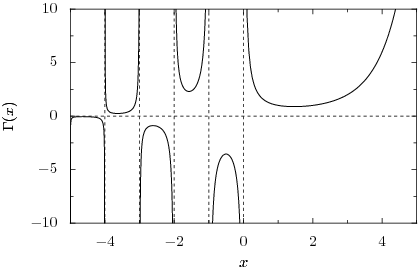
\includegraphics[width=0.5\linewidth]{Gamma_function.png}
    \end{center}
    \caption{Graph of Gamma Function.\cite{gamma}}
    \end{figure}
    
    {\large \url{https://github.com/tavtejS07/SOEN-6011}}
\end{center}

\end{titlepage}

\tableofcontents
\pagebreak

\renewcommand{\thesection}{\arabic{section}}
\section{Problem 3}
\subsection{Algorithms}
\begin{algorithm}
\caption{Lanczos Approximation for StrictMath}
\begin{algorithmic}[1]
\If{$x$ is negative or is $NaN$}
\State $NaN$
\EndIf
\If{$x$ is equal to 0}
\State \textbf{return} $1$
\EndIf
\If{$x$ is greater than 0}
\State $double$ $d = (x-0.5) * log(x+4.5) - (x+4.5)$
\State $double$ $e = 1.0 + X1/(x+0) - X2/(x+1) + X3/(x+2) - $
\State $X4/(x+3) + X5/(X+4) - X6/(x+5)$
\State \textbf{return} $d + log(d1 * sqrt(2*\pi)) --> logGamma$
\EndIf
\State \textbf{Using the value returned in Line 9 calculate $\Gamma(x)$}
\State \textbf{return} $exp(logGamma(x))$

\end{algorithmic}
\end{algorithm}

\begin{algorithm}
\caption{Stirling's Approximation for StrictMath}
\begin{algorithmic}[1]
\If{$x$ is negative or is $NaN$}
\State $NaN$
\EndIf
\If{$x$ is equal to 0}
\State \textbf{return} $1$
\EndIf
\If{$x$ is greater than 0}
\State \textbf{return}
sqrt(2*$\frac{\pi}{x}$)*($\frac{x}{e}$)$^x$
\EndIf
\end{algorithmic}
\end{algorithm}

\subsection{Technical Aspects}
Algorithm 1 is Lanczos approximation of the function $\Gamma(x).$ This is an alternative to the Stirling's approximation. The advantage of this is the less number of single or double floating point precision required. If a real constant is known then we can easily calculate the coefficients in advance and use a single formula.\\
\newline
Algorithm 2 is the approximation of factorials. It has Big Oh! of O(nlogn). Calculation factorial for larger numbers take time if we implement n!. Using the Stirling's approximation it reduces the time of calculation.

\begin{thebibliography}{9}
\addcontentsline{toc}{chapter}{Bibliography}
\bibitem{libretexts}
Libretexts. (2022, February 27). \textit{E14.2: Definition and properties of the gamma function.}Mathematics LibreTexts. Retrieved July 25, 2022, from \texttt{https://math.libretexts.org/Bookshelves/Analysis/\\Complex\_Variables\_with\_Applications\_(Orloff)/14\%3A\_Analytic\_Continuation\_\\and\_the\_Gamma\_Function/14.02\%3A\_Definition\_and\_properties\_of\_the\_Gamma\_function}

\bibitem{gamma}
Gamma function. (2011, July 25). \textit{Gamma function}- Knowino. (n.d.). Retrieved July 27, 2022, from\\ \texttt{https://www.tau.ac.il/~tsirel/dump/Static/knowino.org/wiki/Gamma\_function.html}

\end{thebibliography}

\end{document}